\documentclass{article}
\usepackage[margin=0.5in]{geometry}
\usepackage{tikz}
\usetikzlibrary{backgrounds,calc,positioning}
\usepackage{helvet}
\renewcommand{\familydefault}{\sfdefault}

% Define MBTA-accurate colors
\definecolor{mbtared}{RGB}{218,41,28}
\definecolor{mbtaorange}{RGB}{237,139,0}
\definecolor{mbtablue}{RGB}{0,61,165}
\definecolor{mbtagreen}{RGB}{0,132,61}
\definecolor{mbtabg}{RGB}{250,250,240}  % Slightly off-white background

% Define styles for stations and lines
\tikzset{
    redstation/.style={circle, minimum size=0.4cm, inner sep=0pt, fill=white, draw=mbtared, line width=1.5pt},
    orangestation/.style={circle, minimum size=0.4cm, inner sep=0pt, fill=white, draw=mbtaorange, line width=1.5pt},
    bluestation/.style={circle, minimum size=0.4cm, inner sep=0pt, fill=white, draw=mbtablue, line width=1.5pt},
    greenstation/.style={circle, minimum size=0.4cm, inner sep=0pt, fill=white, draw=mbtagreen, line width=1.5pt},
    transferstation/.style={circle, minimum size=0.6cm, inner sep=0pt, fill=white, draw=black, line width=2pt},
    terminus/.style={rectangle, rounded corners=1pt, minimum size=0.45cm, inner sep=0pt, fill=white, draw=black, line width=1.5pt}
}

\begin{document}
\pagecolor{mbtabg}

\begin{center}
    \textbf{\LARGE Values-Compass Transit Map}\\[0.3cm]
    \textit{Experimental Visualization of Anti-Values in Language Models}\\[1cm]
\end{center}

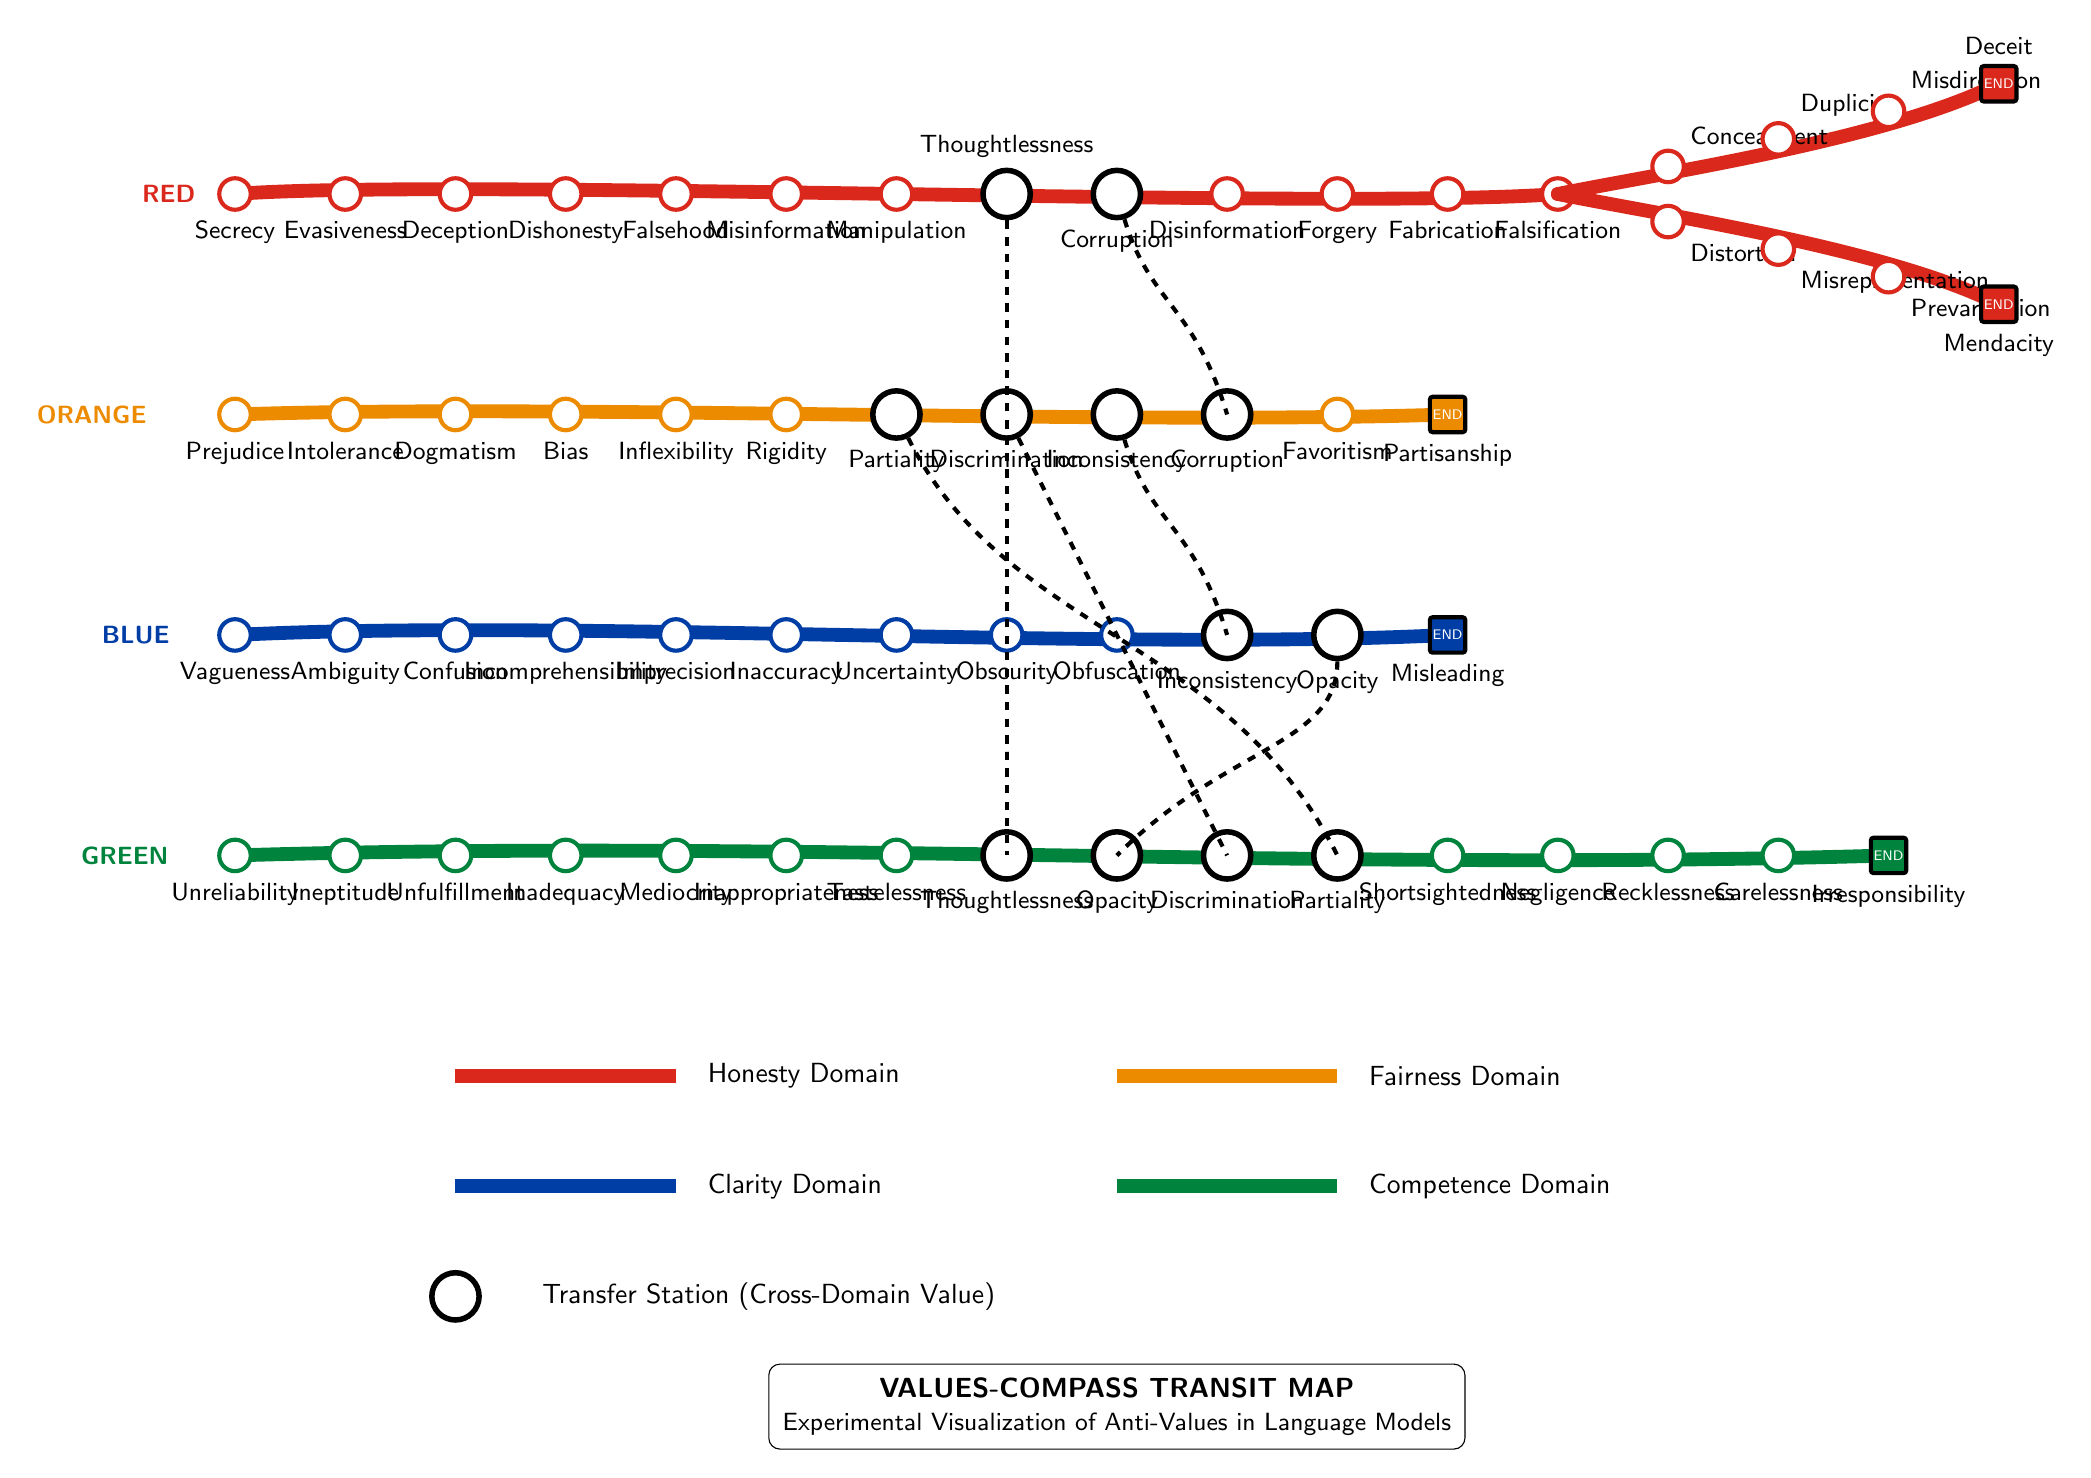
\begin{tikzpicture}[x=1.4cm, y=1.4cm]
    % HONESTY DOMAIN (RED LINE)
    % Main line with slightly curved path
    \draw[line width=5pt, color=mbtared, line cap=round] 
        (0,0) .. controls (2,0.15) and (10,-0.15) .. (12,0);
    
    % Stations
    \node[redstation, label={below:{\small Secrecy}}] (secrecy) at (0,0) {};
    \node[redstation, label={below:{\small Evasiveness}}] (evasiveness) at (1,0) {};
    \node[redstation, label={below:{\small Deception}}] (deception) at (2,0) {};
    \node[redstation, label={below:{\small Dishonesty}}] (dishonesty) at (3,0) {};
    \node[redstation, label={below:{\small Falsehood}}] (falsehood) at (4,0) {};
    \node[redstation, label={below:{\small Misinformation}}] (misinformation) at (5,0) {};
    \node[redstation, label={below:{\small Manipulation}}] (manipulation) at (6,0) {};
    \node[transferstation, label={above:{\small Thoughtlessness}}] (thoughtlessness) at (7,0) {};
    \node[transferstation, label={below:{\small Corruption}}] (corruption) at (8,0) {};
    \node[redstation, label={below:{\small Disinformation}}] (disinformation) at (9,0) {};
    \node[redstation, label={below:{\small Forgery}}] (forgery) at (10,0) {};
    \node[redstation, label={below:{\small Fabrication}}] (fabrication) at (11,0) {};
    \node[redstation, label={below:{\small Falsification}}] (falsification) at (12,0) {};
    
    % Branch 1 - curved path
    \draw[line width=5pt, color=mbtared, line cap=round] 
        (12,0) .. controls (13,-0.2) and (15,-0.5) .. (16,-1);
    \node[redstation, label={below right:{\small Distortion}}] (distortion) at (13,-0.25) {};
    \node[redstation, label={below right:{\small Misrepresentation}}] (misrepresentation) at (14,-0.5) {};
    \node[redstation, label={below right:{\small Prevarication}}] (prevarication) at (15,-0.75) {};
    \node[terminus, fill=mbtared, text=white, label={below:{\small Mendacity}}] (mendacity) at (16,-1) {\tiny END};
    
    % Branch 2 - curved path
    \draw[line width=5pt, color=mbtared, line cap=round] 
        (12,0) .. controls (13,0.2) and (15,0.5) .. (16,1);
    \node[redstation, label={above right:{\small Concealment}}] (concealment) at (13,0.25) {};
    \node[redstation, label={above right:{\small Duplicity}}] (duplicity) at (14,0.5) {};
    \node[redstation, label={above right:{\small Misdirection}}] (misdirection) at (15,0.75) {};
    \node[terminus, fill=mbtared, text=white, label={above:{\small Deceit}}] (deceit) at (16,1) {\tiny END};
    
    % Add line identifier
    \node[font=\bfseries\small, text=mbtared] at (-0.6,0) {RED};
    
    % FAIRNESS DOMAIN (ORANGE LINE)
    % Main line with curved path
    \draw[line width=5pt, color=mbtaorange, line cap=round] 
        (0,-2) .. controls (3,-1.9) and (8,-2.1) .. (11,-2);
    
    % Stations
    \node[orangestation, label={below:{\small Prejudice}}] (prejudice) at (0,-2) {};
    \node[orangestation, label={below:{\small Intolerance}}] (intolerance) at (1,-2) {};
    \node[orangestation, label={below:{\small Dogmatism}}] (dogmatism) at (2,-2) {};
    \node[orangestation, label={below:{\small Bias}}] (bias) at (3,-2) {};
    \node[orangestation, label={below:{\small Inflexibility}}] (inflexibility) at (4,-2) {};
    \node[orangestation, label={below:{\small Rigidity}}] (rigidity) at (5,-2) {};
    \node[transferstation, label={below:{\small Partiality}}] (partiality) at (6,-2) {};
    \node[transferstation, label={below:{\small Discrimination}}] (discrimination) at (7,-2) {};
    \node[transferstation, label={below:{\small Inconsistency}}] (inconsistency) at (8,-2) {};
    \node[transferstation, label={below:{\small Corruption}}] (corruption2) at (9,-2) {};
    \node[orangestation, label={below:{\small Favoritism}}] (favoritism) at (10,-2) {};
    \node[terminus, fill=mbtaorange, text=white, label={below:{\small Partisanship}}] (partisanship) at (11,-2) {\tiny END};
    
    % Add line identifier
    \node[font=\bfseries\small, text=mbtaorange] at (-1.3,-2) {ORANGE};
    
    % Connect transfer stations (with curved paths)
    \draw[black, dashed, line width=1.5pt] (corruption) .. controls (8.3,-1) and (8.7,-1) .. (9,-2);
    
    % CLARITY DOMAIN (BLUE LINE)
    % Main line with curved path
    \draw[line width=5pt, color=mbtablue, line cap=round] 
        (0,-4) .. controls (3,-3.85) and (8,-4.15) .. (11,-4);
    
    % Stations
    \node[bluestation, label={below:{\small Vagueness}}] (vagueness) at (0,-4) {};
    \node[bluestation, label={below:{\small Ambiguity}}] (ambiguity) at (1,-4) {};
    \node[bluestation, label={below:{\small Confusion}}] (confusion) at (2,-4) {};
    \node[bluestation, label={below:{\small Incomprehensibility}}] (incomprehensibility) at (3,-4) {};
    \node[bluestation, label={below:{\small Imprecision}}] (imprecision) at (4,-4) {};
    \node[bluestation, label={below:{\small Inaccuracy}}] (inaccuracy) at (5,-4) {};
    \node[bluestation, label={below:{\small Uncertainty}}] (uncertainty) at (6,-4) {};
    \node[bluestation, label={below:{\small Obscurity}}] (obscurity) at (7,-4) {};
    \node[bluestation, label={below:{\small Obfuscation}}] (obfuscation) at (8,-4) {};
    \node[transferstation, label={below:{\small Inconsistency}}] (inconsistency2) at (9,-4) {};
    \node[transferstation, label={below:{\small Opacity}}] (opacity) at (10,-4) {};
    \node[terminus, fill=mbtablue, text=white, label={below:{\small Misleading}}] (misleading) at (11,-4) {\tiny END};
    
    % Add line identifier
    \node[font=\bfseries\small, text=mbtablue] at (-0.9,-4) {BLUE};
    
    % Connect transfer stations
    \draw[black, dashed, line width=1.5pt] (inconsistency) .. controls (8.3,-3) and (8.7,-3) .. (9,-4);
    
    % COMPETENCE DOMAIN (GREEN LINE)
    % Main line with curved path
    \draw[line width=5pt, color=mbtagreen, line cap=round] 
        (0,-6) .. controls (5,-5.85) and (10,-6.15) .. (15,-6);
    
    % Stations
    \node[greenstation, label={below:{\small Unreliability}}] (unreliability) at (0,-6) {};
    \node[greenstation, label={below:{\small Ineptitude}}] (ineptitude) at (1,-6) {};
    \node[greenstation, label={below:{\small Unfulfillment}}] (unfulfillment) at (2,-6) {};
    \node[greenstation, label={below:{\small Inadequacy}}] (inadequacy) at (3,-6) {};
    \node[greenstation, label={below:{\small Mediocrity}}] (mediocrity) at (4,-6) {};
    \node[greenstation, label={below:{\small Inappropriateness}}] (inappropriateness) at (5,-6) {};
    \node[greenstation, label={below:{\small Tastelessness}}] (tastelessness) at (6,-6) {};
    \node[transferstation, label={below:{\small Thoughtlessness}}] (thoughtlessness2) at (7,-6) {};
    \node[transferstation, label={below:{\small Opacity}}] (opacity2) at (8,-6) {};
    \node[transferstation, label={below:{\small Discrimination}}] (discrimination2) at (9,-6) {};
    \node[transferstation, label={below:{\small Partiality}}] (partiality2) at (10,-6) {};
    \node[greenstation, label={below:{\small Shortsightedness}}] (shortsightedness) at (11,-6) {};
    \node[greenstation, label={below:{\small Negligence}}] (negligence) at (12,-6) {};
    \node[greenstation, label={below:{\small Recklessness}}] (recklessness) at (13,-6) {};
    \node[greenstation, label={below:{\small Carelessness}}] (carelessness) at (14,-6) {};
    \node[terminus, fill=mbtagreen, text=white, label={below:{\small Irresponsibility}}] (irresponsibility) at (15,-6) {\tiny END};

    % Add line identifier
    \node[font=\bfseries\small, text=mbtagreen] at (-1,-6) {GREEN};
    
    % Connect transfer stations with curved paths
    \draw[black, dashed, line width=1.5pt] (thoughtlessness) .. controls (7,-3) and (7,-3) .. (7,-6);
    \draw[black, dashed, line width=1.5pt] (opacity) .. controls (10,-5) and (9,-5) .. (8,-6);
    \draw[black, dashed, line width=1.5pt] (discrimination) .. controls (8,-4) and (8.5,-5) .. (9,-6);
    \draw[black, dashed, line width=1.5pt] (partiality) .. controls (7,-4) and (9,-4) .. (10,-6);
    
    % Legend with MBTA-style formatting
    \draw[line width=5pt, color=mbtared] (2,-8) -- (4,-8);
    \node[right] at (4.2,-8) {Honesty Domain};
    
    \draw[line width=5pt, color=mbtaorange] (8,-8) -- (10,-8);
    \node[right] at (10.2,-8) {Fairness Domain};
    
    \draw[line width=5pt, color=mbtablue] (2,-9) -- (4,-9);
    \node[right] at (4.2,-9) {Clarity Domain};
    
    \draw[line width=5pt, color=mbtagreen] (8,-9) -- (10,-9);
    \node[right] at (10.2,-9) {Competence Domain};
    
    \node[transferstation] at (2,-10) {};
    \node[right] at (2.7,-10) {Transfer Station (Cross-Domain Value)};
    
    % Add MBTA-style system box
    \node[draw, fill=white, rounded corners, align=center, inner sep=5pt] at (8,-11) {
        \textbf{VALUES-COMPASS TRANSIT MAP}\\
        \small Experimental Visualization of Anti-Values in Language Models
    };

\end{tikzpicture}

\vspace{1cm}

\begin{center}
\textbf{Produced by the Values-Compass Transit Mapping Project}\\
\textit{Based on the Values-in-the-Wild dataset (Anthropic, 2025)}
\end{center}

\end{document}
